\subsection{Structured-Control-Flow Construct}

Translating from stack-based IR to register-based IR is not trivial, especially when non-linear control flow structures appeared. This problem appeared in many runtime system implementations, such as Numba \cite{numba}, a just-in-time (JIT) compiler for Python. Usually, one needs some algorithm to recover the control flow structure from annoying jump instructions. Luckily, in WebAssembly, we can translate the stack-based bytecode into register-based basic blocks in linear time, thanks to the structured-control-flow constructs and their validation rules defined in WebAssembly. In this section, we will cover the translation pattern used for WebAssembly's structured-control-flow constructs, namely \texttt{block}, \texttt{if} and \texttt{loop}.

\begin{figure}
  \centering
  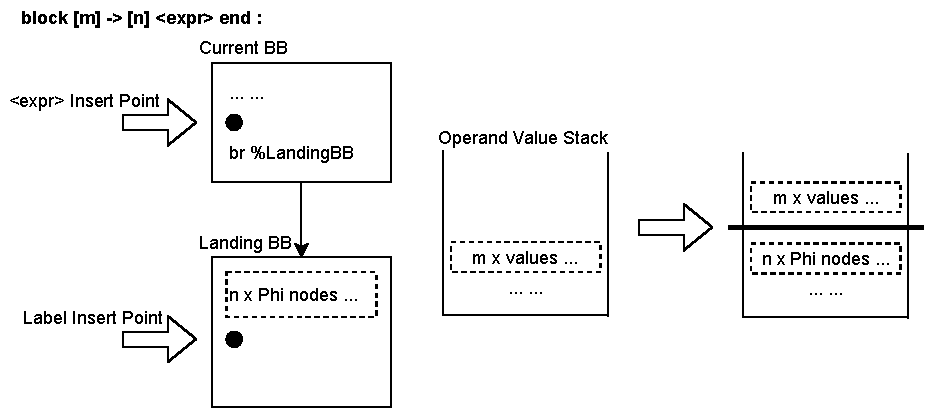
\includegraphics[width=\textwidth]{Images/4.MIR/translate-block.pdf}
  \caption{WebAssembly \texttt{block} translation pattern}
  \label{fig:translate-block}
\end{figure}

\begin{figure}
  \centering
  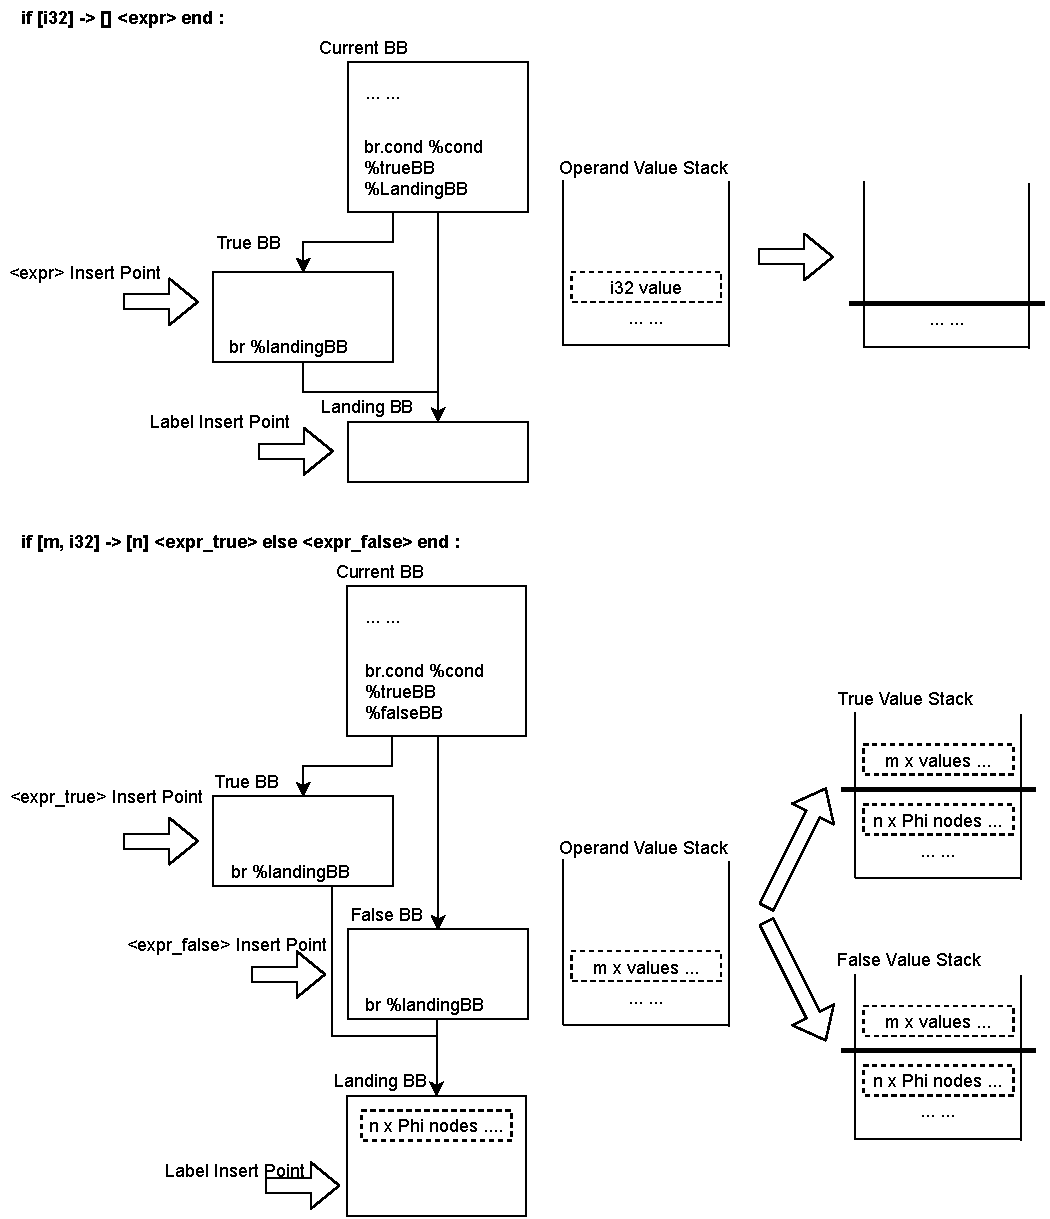
\includegraphics[width=\textwidth]{Images/4.MIR/translate-if.pdf}
  \caption{WebAssembly \texttt{if} translation pattern}
  \label{fig:translate-if}
\end{figure}

\paragraph{Block} In the background chapter, we provide a general illustration of the three structured-control-flow constructs.  As a quick recap, \texttt{block} is the simplest form of a structured-control-flow construct. It implicitly introduces a label at the end of its enclosing instructions. A branching instruction referring to this label will redirect the control flow to the end of the block. Figure~\ref{fig:translate-block} illustrates the translation pattern for WebAssembly \texttt{block} in SableWasm MIR.  We will first clarify some of the terminologies we used in the figure, and we will use the same terms later in the \texttt{loop} and \texttt{if} pattern discussion. \emph{Expr Insert Point} refer to the starting position for the generated instructions when we recursively translate the instructions within the enclosing expression of the \texttt{block} instruction. Furthermore, \emph{Label Insert Point} refer to the position for generated instruction when we finish the recursive translation and resume to the parent expression of the \texttt{block} instruction. A \emph{label stack entry} is a tuple consisting of a pointer to the landing BB, a list of Phi nodes expecting merge values, and a pointer to the \emph{label insert point}. The translation pattern for \texttt{block} is pretty simple; we continue on the current BB and prepare the landing BB for the block instruction as the branch instructions within the nested expression may refer to the label. Additionally, to fully support multi-value extension in WebAssembly, we need also to prepare the Phi nodes in the landing BB. SableWasm generates the Phi nodes from the type of the \texttt{block} instruction. WebAssembly validation ensures that the nested expression can access exactly $m$ values from the stack and put $n$ values onto the stack. Finally, we will append an unconditional branching to the landing BB because in WebAssembly, if the control flow reaches the bottom of the \texttt{block} expressions, it will implicitly fall through. For operand stack, we will first pop $m$ values from the stack as \texttt{block} instruction's type suggests and push the Phi nodes as the result values. Now we need to set up the operand stack for our nested expression. Again, due to the WebAssembly validation rule, we need to insert a boundary before continuing. Figures~\ref{fig:translate-block} represents this with the bold line in the result operand value stack. We create a new operand value-stack during recursive translation instead of using some magic stack elements in practice.  Because the nested can access $m$ values from the parent stack, finally, we push the $m$ values onto the new stack.


\paragraph{If} The next control-flow structure defined WebAssembly in \texttt{if}. \texttt{if} is very similar to a \emph{if} statement that appears in many other programming languages. Figure~\ref{fig:translate-if} illustrates the translation patterns that used in SableWasm. There are two types of \texttt{if} instruction defined in WebAssembly specification. The first case is a partial \texttt{if} instruction, where it only contains the `true' branch. From WebAssembly validation rules, it's easy to show that the only possible type is \texttt{[i32]->[]}, even with the multi-value extension proposal. Hence, the translation pattern or the partial \texttt{if} is quite straightforward. In the current BB, we only need to pop the condition value from the operand stack and construct a conditional branch based on this value. On the other hand, we also have `full' \texttt{if} instructions with both true expression and false expression. The validation rules ensure that both expressions will have the same type. The translation pattern is relative more complex compare to that of a partial \texttt{if}. In this case, we have to prepare the landing BB similarly as we did for the \texttt{block} construct. We need to generate $n$ Phi nodes for data-flow mergers from the true branch, the false branch, and any possible branching instruction within both nested expressions. Similarly, we need to pop $m$ values from the stack for operand values stack and then push $n$ Phi Nodes. And, within both nested expressions, push $m$ values back to the stack.

\begin{figure}
  \centering
  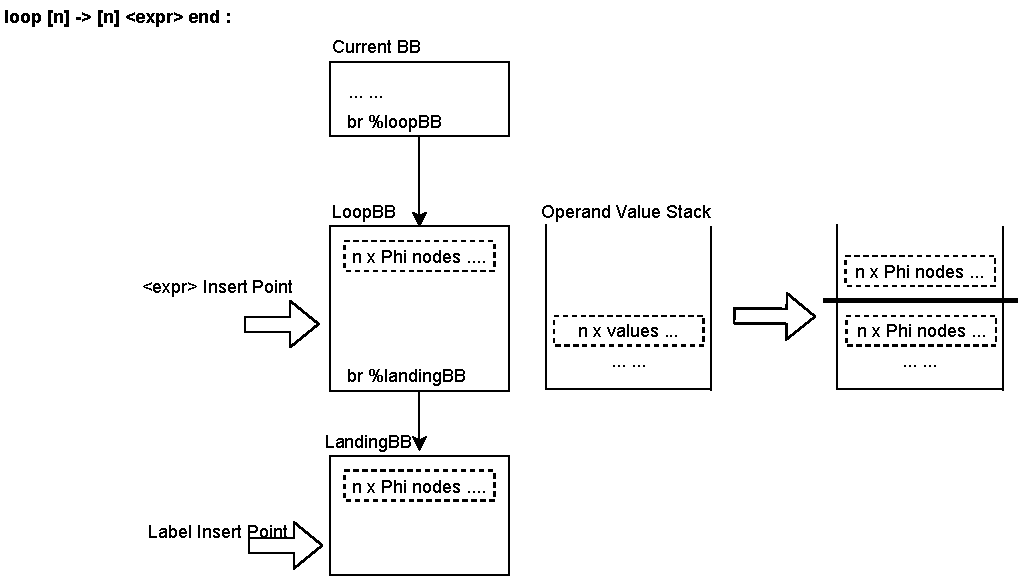
\includegraphics[width=\textwidth]{Images/4.MIR/translate-loop.pdf}
  \caption{WebAssembly \texttt{loop} translation pattern}
  \label{fig:translate-loop}
\end{figure}

\paragraph{Loop} The last control-flow structure defined in WebAssembly is \texttt{loop}. Figure~\ref{fig:translate-loop} gives a general illustration of SableWasm's translation pattern for \texttt{loop} instructions. Similar to the partial \texttt{if} we discussed in the previous paragraph, one can show that, under WebAssembly's validation rules, the parameter types for \texttt{loop} instruction must equal to the result types. \texttt{loop} instruction is similar to the \texttt{block} instruction, except that if any branching instruction refers to it, the branching instruction should transfer the control flow to the beginning of the expression instead of the end. Thus, we need to prepare a standalone basic block for the nested expression in \texttt{loop}, along with the Phi Nodes. Note that we also introduce Phi nodes in the landing BB. One may argue that there is no need for these Phi nodes, as the control flow is determined and no value merging will occur. Indeed, these Phi nodes will always be trivial Phi nodes, which have only one possible value inflow. However, this is due to the limitation of our translation framework. In the \texttt{block} paragraph, we mentioned that instead of using magic stack elements to signal separation between scopes, we create a new stack for each nested expression. Further, the recursive translation visitor will discard its operand stack once it finishes translation. Thus, there is no possible way in the SableWasm MIR translation framework to access the operand stack from nested expression translation. To alleviate the problem, we create these Phi nodes ahead of nested expression translation, and later we can add candidate values to them to achieve the same effect. This method is sub-optimal and adds unneeded complexity to the translated control-flow graph. We will come back to this problem later in the chapter when we discuss control-flow graph simplification.

In this section, we discussed the translation patterns for WebAssembly structured control-flow constructs. Thanks to WebAssembly validation rules, the types for these structured control-flow instructions explicitly mark value merging and imply possible Phi nodes. Furthermore, one can show that the control graph generated above is indeed in SSA and within linear time. However, the directly generated control flow graph is not easily understandable by users. This mainly comes from two facts. First, the WebAssembly-targeting compiler may generate awkward patterns to fit in the structured control-flow constructs. Second, SableWasm translation patterns for structured-control flow constructs is clearly not optimal.